% Constructed illustration, not a solver output or benchmark result.
\begin{figure}[pos=H]
\centering
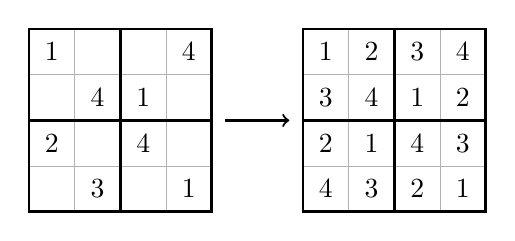
\begin{tikzpicture}[scale=0.58]
 \foreach \offset in {0,6} {
  \begin{scope}[xshift=\offset cm]
   \draw[step=1,gray!60,thin] (0,0) grid (4,4);
   \draw[line width=1pt] (0,0) rectangle (4,4);
   \draw[line width=1pt] (2,0)--(2,4) (0,2)--(4,2);
  \end{scope}
 }
 \foreach \x/\y/\v in {0/0/1,3/0/4,1/1/4,2/1/1,0/2/2,2/2/4,1/3/3,3/3/1}
  \node[text=black] at (\x+0.5,3.5-\y) {$\v$};
 \foreach \r/\vals in {0/{1,2,3,4},1/{3,4,1,2},2/{2,1,4,3},3/{4,3,2,1}}
  \foreach \v [count=\c from 0] in \vals
   \node[text=black] at (6.5+\c,3.5-\r) {$\v$};
 \draw[->,thick] (4.3,2)--(5.7,2);
\end{tikzpicture}
\caption{\lang{Ví dụ $4\times4$: input (trái) và một cách hoàn thành (phải) dựng để minh họa; không phải output solver hoặc chứng nhận uniqueness.}{A $4\times4$ input (left) and a constructed completion (right), for illustration; not solver output or a uniqueness certificate.}}
\label{fig:example4}
\end{figure}
